\section{Hadoop MapReduce to Spark}
\label{sec:history}
In several Big Data mining tools that have been developed, the most notable ones are MapReduce and Spark. MapReduce is a cluster computing framework 
which supports locality-aware scheduling, fault tolerance, and load balancing. Spark improves operations that MapReduce does not cover well. 

MapReduce provides a programming model where the user creates acyclic data flow graphs to pass input data through a set of operations. This 
data flow programming model is useful for many of query applications. However, MapReduce framework struggles from two of main resent data mining jobs: iterative jobs and interactive analysis. 

Iterative job is especially common in Machine Learning Algorithm, such as Gradient Descent. In traditional MapReduce framework, each iteration can be expressed as single MapReduce job 
so that each job must reload the data from disk. This leads I/O overhead and deteriorates performance of iterative algorithms. 

Interactive analysis is also an inevitable task in modern data science. A data scientist want perform exploratory analysis in interactive way. 
Nevertheless, MapReduce is designed in the way more stable for ad-hoc query, so each analysis can be single MapReduce job. 
To perform multiple analysis to explore dataset, the data needs to be written to and reload from disk many times. 

To overcome these limitations, Spark has been developed as a new cluster computing framework maintaining the innovative characteristics of MapReduce and improving 
its iterative and interactive jobs with in-memory data structure.


\section{Resilient Distributed Datasets}
\label{sec:history}
The major methods in Spark are Resilient Distributed Datasets (RDDs), a data structure that abstracts distributed memory across different clusters. 
The immutable coarse-grained transformation, spark-scheduler with lazy-evaluation, and memory management with cacheing achieve computation with fault-tolerance, 
fast execution, and moderate control on memory efficiency \cite{DBLP:conf/nsdi/ZahariaCDDMMFSS12}.

A RDD is essentially a multi-layer Java data structure. A top RDD object references Java array, which intern, references a set of tuple objects. 
The coarse-grained transformations and immutability requires a RDD to be deep-copied to produce a new RDD, but efficiently offers fault tolerance. 
The lost partitions of a RDD can be recomputed in parallel on different nodes rather than rolling back the whole program.

Spark-pipeline consists of sequence of transformations and actions over RDDs. A transformation produces a new RDD from a set of existing RDD. 
An action is method that computes statistics from an RDD. Due to lazy-evaluation nature, transformations do not materialize the newly created RDD. 
Instead, RDD Lineages are created. Lineage is a graph among parent and child RDDs which represents logical execution plan. 
This enhance fault-tolerance and improve ability to optimize execution plan. 

RDDs can be cached in memory for faster access by persist method. Developers can specify a storage level for a persisted RDD, in memory with serialized or deserialized, or on disk. 
Other than persisted RDD, Spark generates a lot of intermediate RDDs during execution. Since RDD is a Java object, they are managed by Garbage Collection (GC) in the JVM. 
However, persisted RDDs are never collected by GC. This GC might cause significant deterioration of performance of Spark, because GC shows heavy overhead when there are a number of objects.


\section{Memory Management in Spark}
\label{sec:history}
Spark framework allocates multiple executors, JVMs, that run sequence of transformations and actions. As we describe the previous section, data in Spark is mainly stored as Java objects in memory, 
so that they are allocated on JVM heap and managed by JVM Garbage Collection. The data may form three types \cite{DBLP:journals/pvldb/XuGDWW19}: Cached data, Shuffled data, and Operator-generated data. 

Spark can cache data in memory to reduce disk I/O. This Cached data usually long-lived Java objects and span multiple stages in Spark-pipeline. 
Spark allocates a logical storage space to store the cached data as shown in Figure. After aggregation, Spark generates Shuffled data. Shuffled data is usually long-lived, 
because it need to be kept in memory until the task ends. Spark allocates execution space to store Shuffled data.
The storage space and execution space spans 60 \% of JVM heap space in default. Operator-generated data is data generated by user-defined operations. Since Operator-generated data may or may not be used, 
after the operation finish, the data object can be both short-lived or long-lived objects. These are stored in user space allocated on default 40 \% of JVM heap.

All data of these types on JVM heap is managed by JVM GC. GC check references graph of objects, mark whether the objects are used and deallocate memory space occupied by unused objects. 
There are three popular GCs: Parallel, CMS and G1. All of these method track generation of object based on the region of memory. 
The Java logical heap structure is shown in Figure. It can be separated into three main parts where store objects for each corresponding generation: 
permanent generation, young generation, and old generation. The region for permanent generation stores metadata required by JVM to describe 
class and method used in application which will be permanently lived on the region of memory. 

The region for young generation mainly consists of two parts: Eden and Survivor space. 
First, Java objects are created in Eden space and promoted to Survivor space when survive from GC. 
After objects survive several GCs in Survivor space, they are finally promoted to old generation.

In old generation, JVM lunches multi-thread to perform GC. GC with multi-threading suffers from Stop-The-World (STW) pauses; 
GC may suspend application threads while performing object marking and deallocation. 
Different GC algorithms try to solve this problem with trade-off between GC frequency and memory utilization. 

Because of the problem of STW and copying objects to different physical memory pages , JVM GC cause huge overhead when number of objects is large. 
Therefore, GC become severe issue in Big Data processing where might produce significant number of object.

\begin{figure}[htb]
    \includegraphics[width=15cm]{java_heap.eps}
    \caption{Java Heap Structure}
    \label{fig:Sampling}
\end{figure}

\begin{figure}[htb]
    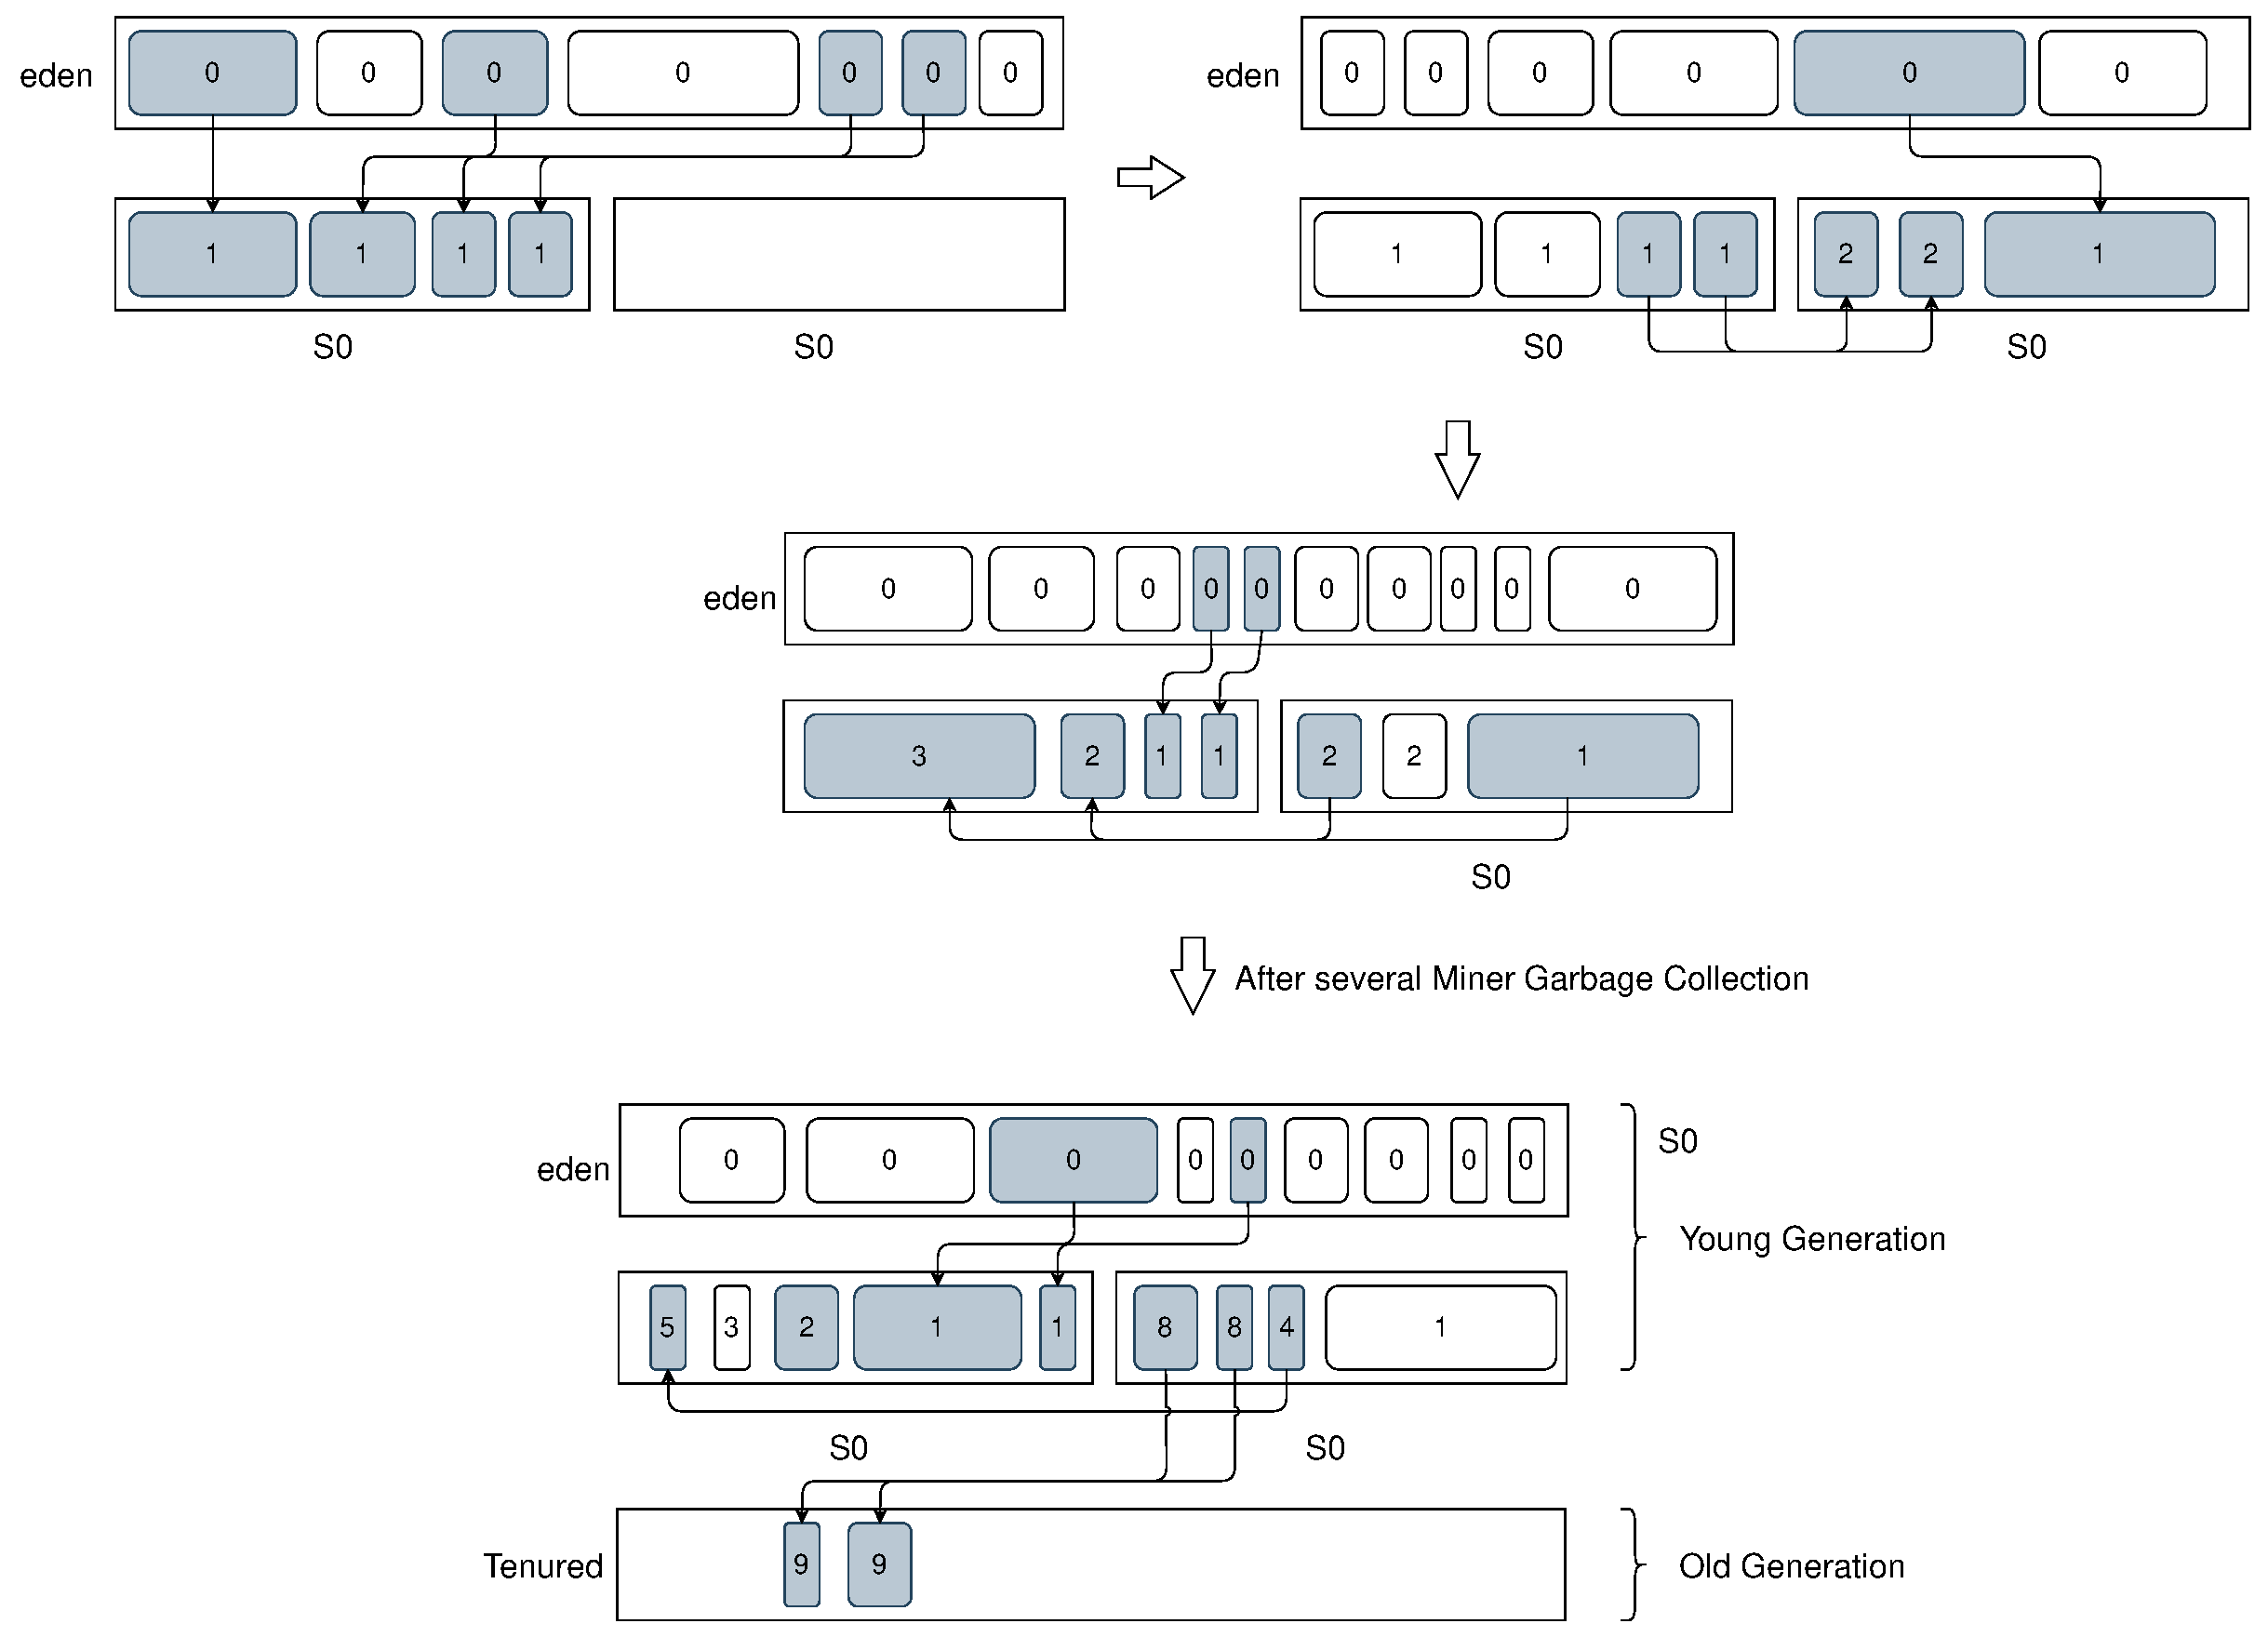
\includegraphics[width=15cm]{java_gc.eps}
    \caption{Java Garbage Collection}
    \label{fig:Sampling}
\end{figure}



\begin{itemize}
    \item GC tuning solutions
    \item Annotation, off-heap solution 
\end{itemize}



\section{Application to System Language}
\label{sec:history}


